\documentclass[draftcls, onecolumn, journal]{IEEEtran}
% \documentclass[journal]{IEEEtran}
% \documentclass[inproceedings]{article}
%\usepackage{fullpage}

%\renewcommand{\baselinestretch}{1.9}
\usepackage{graphicx}
%\usepackage{cite}
\usepackage[style=ieee, nohashothers=true, nosortothers=true, uniquelist=true, natbib=true, backend=biber, sorting=none]{biblatex}
\DefineBibliographyStrings{english}{andothers={}}

\addbibresource{project.bib}
\DeclareFieldFormat[article]{volume}{Vol. #1}
\DeclareFieldFormat[article]{number}{No. #1}
\DeclareFieldFormat[article]{pages}{p. #1}
\DeclareFieldFormat[inproceedings]{pages}{p. #1}

%\documentclass[journal]{IEEEtran}
\usepackage[a4paper, total={6in, 8.5in}, top=1in, bottom=1in, left=1in, right=1in]{geometry}
\usepackage{mathtools}
\usepackage{amssymb}
\usepackage{amsmath}
\usepackage{pythonhighlight}
\usepackage[utf8]{inputenc}
\usepackage{fancyhdr}
\usepackage{pythonhighlight}
\usepackage{changepage}
\usepackage{slashbox}
\usepackage{floatrow}
\usepackage{listings}
\usepackage[hidelinks]{hyperref}
\usepackage[T1]{fontenc}
\usepackage[utf8]{inputenc}
\usepackage[english]{babel}
\usepackage{csquotes}
\usepackage{booktabs}
\usepackage{multicol}
\usepackage{titlesec}
\usepackage{fontawesome5}
\usepackage{makecell}
\usepackage{footnote}
\usepackage{hyperref}

\setcounter{secnumdepth}{4}
\setcounter{tocdepth}{4}


\titleformat{\paragraph}
{\normalfont\normalsize\bfseries}{\theparagraph}{1em}{}
\titlespacing*{\paragraph}
{0pt}{3.25ex plus 1ex minus .2ex}{1.5ex plus .2ex}

\usepackage{caption}
\usepackage{subcaption}
\usepackage{color} %red, green, blue, yellow, cyan, magenta, black, white
\definecolor{mygreen}{RGB}{28,172,0} % color values Red, Green, Blue
\definecolor{mylilas}{RGB}{170,55,241}


\floatsetup[table]{capposition=top}

\sloppy
\definecolor{lightgray}{gray}{0.5}
\setlength{\parindent}{0pt}
\setlength{\headheight}{14pt}

\renewcommand{\headrulewidth}{.4mm} % header line width
\newcommand{\norm}[1]{\left\lVert#1\right\rVert}
\renewcommand\footnoterule{\kern-3pt \hrule width 3in \noindent \kern 2.6pt}


\pagestyle{fancy}
\fancyhf{}
\fancyhfoffset[L]{1cm} % left extra length
\fancyhfoffset[R]{1cm} % right extra length
\rhead{\bfseries Kutay U\u{g}urlu 2232841}
\lhead{ADPC for Tikhonov Regularization Parameter Choice}
\rfoot{}

\DeclarePairedDelimiter\ceil{\lceil}{\rceil}
\DeclarePairedDelimiter\floor{\lfloor}{\rfloor}

\author{Kutay U\u{g}urlu 2232841}

\begin{document}

    
\lstset{language=Matlab,%
    %basicstyle=\color{red},
    breaklines=true,%
    morekeywords={matlab2tikz},
    keywordstyle=\color{blue},%
    morekeywords=[2]{1}, keywordstyle=[2]{\color{black}},
    identifierstyle=\color{black},%
    stringstyle=\color{mylilas},
    commentstyle=\color{mygreen},%
    showstringspaces=false,%without this there will be a symbol in the places where there is a space
    numbers=left,%
    numberstyle={\tiny \color{black}},% size of the numbers
    numbersep=9pt, % this defines how far the numbers are from the text
    emph=[1]{for,end,break},emphstyle=[1]\color{red}, %some words to emphasise
    %emph=[2]{word1,word2}, emphstyle=[2]{style},    
}

\fancyfoot[C]{\thepage}

\title{\LARGE \LARGE EE798 Remote Image Formation Theory Project \newline \newline
Analysis and Reimplementation of \newline \textit{Improving the spatial solution of electrocardiographic
imaging: A new regularization parameter choice
technique for the Tikhonov method}}

\maketitle{\LARGE}
\pagebreak
\tableofcontents
\listoffigures
\listoftables
\pagebreak

\section{Introduction}

\indent Electrocardiographic Imaging (ECGI) is a noninvasive method for reconstructing the epicardial potentials from the body surface potential mapping that can diagnose diseases such as tachycardia \cite{intini2005electrocardiographic} and atrial fibrillation \cite{figuera2016regularization,schuler2017ecg}. The number of measurement non-invasively taken from the torso surface, however, is less than the number of reconstructed cardiac sources that provides satisfactory spatial resolution for the diagnosis. Due to the inherent ill-posedness of this underdetermined problem, utilization of regularization is mandatory to achieve physiologically suitable solutions \cite{milanivc2014assessment}. Tikhonov Regularization is a widely used regularization technique in ECGI community and has been found to outperform the other methods depending on the formulation of the problem \cite*{milanivc2014assessment}. The regularization technique imposes a prior on the inverse problem solution and weights the candidate solutions with the data-fidelity term in the cost function with a regularization parameter $\lambda$. Chamorro-Servent, \textit{et al.}, proposes a new method called Automated Discrete Picard Condition(ADPC) in their study \cite*{chamorro2017improving} to automatically find a suitable regularization parameter $\lambda$. 
This project report investigates the idea reported in \textit{Improving the spatial solution of electrocardiographic
imaging: A new regularization parameter choice technique for the Tikhonov method}~\cite{chamorro2017improving}.  
\\
\\
The organization of the report is as follows:
\begin{itemize}
    \item The problem and the proposed solutions to it are briefly introduced in this section.
    \item The background of ECGI and theory of the regarding inverse problem are discussed in Section \nameref{sec:theory}.
    \item The methods, datasets and the details regarding the implementation of proposed methods for both the original study and the reimplemented version with another experimental setup are shared in the \nameref{sec:implementation} section.
    \item Section \nameref{sec:discussion} is left for the presentation of the results from conducted experiments along with the original results presented in the study and the discussion comparing the performances of the related method.
\end{itemize}

\clearpage

\section{Theory}\label{sec:theory}

\begin{figure}[h]
    \centering
    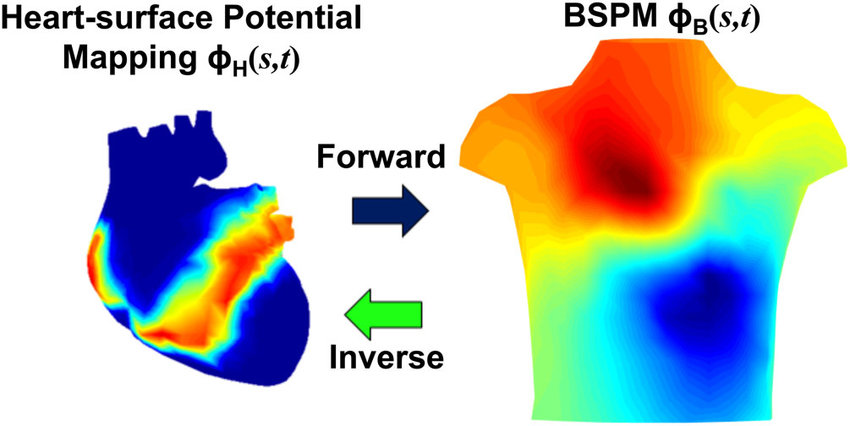
\includegraphics[width=0.8\textwidth]{../images/The-illustration-of-forward-and-inverse-ECG-problems.png}
    \caption{ECGI Forward and Inverse Problem}\label{fig:ECG}
\end{figure}

\subsection{ECGI Forward Problem}\label{subsec:ecgfor}

\indent ECGI Forward problem is constructing a model for calculating the body surface potential mapping(BSPM) from the given heart potentials, \textit{i.e.}, the epicardial voltage distribution, shown by the right-side arrow in Figure \ref{fig:ECG}. One can come up with different forward models for the ECGI problem. The authors of the original study utilized Method of Fundamental Solutions(MFS) method to derive the forward model, whereas Boundary Element Method(BEM) is utilized for the re-implementation. 

\subsubsection*{Method of Fundemental Solutions}
\indent MFS is meshless approach adapted to ECGI. In this method, the measurements are expressed as a linear combination of fundamental solutions to the LapLace equation. It is formulated as

\begin{equation}
    \Phi (x) = a_0 + \sum\limits_{j=1}^{N_s} f(x-y_j)a_j
    \label{eq:MFS}
\end{equation}

where $x \in \Omega$ where $\Omega$ is the measurement domain (torso) and $y_j$'s are the $N_s$ locations of the sources ($y_j \notin \Omega$) (heart). In this formulation $f$ stands for the fundemental solution to LapLace equation in Eqn. \ref{eq:FundSoln}:

\begin{equation}
    f(r) = \frac{1}{4\pi} \frac{1}{|r|}
    \label{eq:FundSoln}
\end{equation}

After the discretization of the domain on torso measurement locations, the following system matrix M can be obtained:

\begin{center}
    $M = \begin{bmatrix} 
        1 & f(r_{11}) & \dots & f(r_1 N_S) \\
        \vdots & \vdots  & \ddots & \vdots\\
        1 &  f(r_{N_T1}) & \dots & f(r_{N_T} N_S) \\ 
        0 & \partial_{n_1}f(r_{11}) & \dots & \partial_{n_1}f(r_1 N_S) \\
        \vdots & \vdots  & \ddots & \vdots\\
        0 &  \partial_{n_{N_T}}f(r_{N_T1}) & \dots & \partial_{n_{N_T}}f(r_{N_T} N_S)     
        \end{bmatrix}$    
\end{center}

\subsection{ECGI Inverse Problem}\label{subsec:ecginv}

\subsection{Tikhonov Regularization}\label{subsec:tikreg}

\subsection{Parameter Choice Techniques}\label{subsec:paramselect}

\section{Implementation}\label{sec:implementation}


\section{Results}\label{sec:results}
\section{Results and Discussion}\label{sec:discussion}

\printbibliography
\end{document}